\Lecture{Jayalal Sarma}{Sept 29, 2020}{08}{PIE and three applications}{Sumanth Naik}{$\alpha$}{JS}

%\section{Introduction}
The journey so far has been that we have been doing counting by bijections and established certain ideas regarding double counting and the bijections behind the scenes. Then we came to Principle of Inclusion-Exclusion(PIE) as a consequence of a bijection argument. In this lecture, we will look at another proof (an algebraic proof) for PIE and then 3 interesting applications of PIE.

\section{Principle of Inclusion Exclusion (PIE) - An Algebraic Proof} \label{sec:Principle of Inclusion - Exclusion(PIE)}
If there are $n$ subsets of a ground set $X$; $A_1$, $A_2$, $A_3, \ldots A_n$ $\subseteq$ $X$, then PIE helps us to estimate the size of the set of union of all $n$ subsets of the ground set. Mathematically, PIE states that,
\begin{align*}
\left|\bigcup_{i=1}^{n} A_i\right| &= \sum_{1 \le i \le n} | A_i|
\hspace{0.1cm}- \sum_{1 \le i < j \le n} \left| A_i \cap A_j \right| \\
&\hspace{0.5cm}+ \sum_{1 \le i < j < k \le n} | A_i \cap A_j \cap A_k| \hspace{0.2cm}.\hspace{0.1cm}.\hspace{0.1cm}.\hspace{0.1cm}.\hspace{0.1cm}.\\
\left|\bigcup_{i=1}^{n} A_i\right| &= \sum_{\emptyset \neq I \subseteq [n]} (-1)^{|I| +1} \left|\bigcap_{i \in I} A_i \right|\\
&=\sum_{\emptyset \neq I \subseteq [n]} (-1)^{|I| +1} \left|A_I\right|
\end{align*}
where $[n] = \{1,2,3, \ldots, n\} $ (short-hand notation for $1$ to $n$ elements) and $A_I = \bigcap_{i \in I} A_i$.\\
\\
Note that the intuition behind understanding the formula in the second step from first is that, $ \emptyset \neq I \subseteq [n]$ captures all the combinations of $1,2,3, \ldots ,n$ sized sets from $n$ sized set of numbers, i.e., $1 \le i \le n$ (set of combinations of 1 sized set from n sized set), $1 \le i < j \le n$ (set of combinations of 2 sized set from n sized set) and so on up to set of combinations of $n$ sized set from n sized set. The alternating sign in first equation's term is captured by $(-1)^{|I| +1}$ in second equation. And finally, the intersection part of all the terms in first equation, i.e., $|A_i|, |A_i \cap A_j|,  |A_i \cap A_j \cap A_j| \ldots$ is captured in $ \bigcap_{i \in I} A_i$ of the second equation.
\begin{proof}
Define the characterestic function of the set $A_i$ as $f_i$ described as : $f_i:X\longrightarrow\{0,1\}$, where the images are defined as $$\forall x \in X,\hspace{0.3cm} f_i(x) = 
  \begin{cases}
    1&\mbox{if } x \in A_i \\
    0& \textrm{otherwise }
  \end{cases}
$$

By definition, $(1-f_i(x))$ is the characteristic function for the compliment of $A_i$ (i.e. $X\setminus A_i$ or $\overline A_i$). In other words, when you subtract the characteristic function of a set from $1$, the difference is the characteristic function of the compliment of the same set. It is also to be noted that $f_i(x)f_j(x)$ is the characteristic function of $A_i\cap A_j$. In other words; when you multiply the characteristic functions of two sets with each other, the product is the characteristic function of the intersection of the two sets. 
\begin{align}
\intertext{Consider a function defined as,} F(x) &= \prod_{i=1}^{n}(1-f_i(x))\nonumber \\
&= (1-f_1(x))(1-f_2(x)) \ldots (1-f_n(x))\nonumber  \\
&= \sum_{I\subseteq[n]}(-1)^{|I|}\left(\prod_{i \in I} f_i(x)\right) \label{eq:F_def_in_PIE}
\end{align}
Note that the $F(x)$ represents the characteristic function of intersection of compliments (compliment of each $f_i$), hence by De-Morgan's Law, its mathematical equivalent is,
\[
\overline{\left(\bigcup_{i=1}^{n} A_i\right)} = X \setminus \bigcup	_{i=1}^{n}A_i
\]
To get the size of the set in the $RHS$ of previous equation (it has all the elements which are not present in any of the $n$ subsets of $X$), we just need to count the number of $x$'s in $X$ for which $F(x)$ is 1 (as $F(x)$ will be 1 for any $x$ only if every $f_i(x)$ is 0, i.e., $\forall i,x \notin A_i$). Hence:
\begin{equation}
\label{eq:sigma_F_1}
|X \setminus \bigcup_{i=1}^{n}A_i| = \sum_{x \in X} F(x) 
\end{equation}

Also from (\ref{eq:F_def_in_PIE}),
\begin{align}
\sum_{x \in X} F(x)&= \sum_{x} \sum_{I \subseteq [n]} (-1)^{|I|} \left(\prod_{i \in I} f_i(x)\right)\nonumber \\
&= \sum_{I \subseteq [n]} (-1)^{|I|} \left(\sum_{x} \left(\prod_{i \in I} f_i(x)\right)\right)\nonumber \\
&=\sum_{I \subseteq [n]} (-1)^{|I|} \left|\bigcap_{i \in I}A_i\right|\label{eq:sigma_F_2}
\end{align}
The last step is because $(\prod_{i \in I} f_i(x))$ is the characteristic function of intersection of $n$ subsets, i.e., $\bigcap_{i \in I}A_i$. And its summation over $x$, $(\sum_{x} (\prod_{i \in I} f_i(x)))$ will give us the size of the intersection, $\left|\bigcap_{i \in I}A_i\right|$. Also, note that the convention when $I=\emptyset$ is,
%\begin{equation}
$\left|\bigcap_{i \in I}A_i\right| = |X|$.
which can be reasoned as when $I$ is empty, $\left(\prod_{i \in I} f_i(x)\right)$ is $1$ for any $x$. And its summation over $x$, $\sum_{x} \left(\prod_{i \in I} f_i(x)\right)$ gives $|X|$.
\begin{align*}
\intertext{By (\ref{eq:sigma_F_1}) and (\ref{eq:sigma_F_2}),}
\left|X \setminus \bigcup_{i=1}^{n}A_i\right| &= \sum_{I \subseteq [n]} (-1)^{|I|} \left|\bigcap_{i \in I}A_i\right|\\
|X | - \left| \bigcup_{i=1}^{n}A_i\right| &= \sum_{I \subseteq [n]} (-1)^{|I|} \left|\bigcap_{i \in I}A_i \right|\\
\left| \bigcup_{i=1}^{n}A_i \right| &= |X| - \sum_{I \subseteq [n]} (-1)^{|I|} \left|\bigcap_{i \in I}A_i\right|\\ 
&=\sum_{\emptyset \neq I \subseteq [n]} (-1)^{|I|+1} \left|\bigcap_{i \in I}A_i \right| \\
\end{align*}
This completes the algebraic proof for PIE.
\end{proof}


\section{Applications of PIE} \label{sec:Applications of PIE - lec1}

We now see three different applications of PIE which exposes some interesting features of the tool.

\subsection{Counting the number of derangements on $n$ elements.} \label{subsec:derangements application}
Consider a scenario where, $n$ people go to a theatre to watch a movie, they keep their hats outside with the gatekeeper. On return, in a rush, the gatekeeper panicked and gave back the hats randomly.\\
\textbf{Question:} What is the chance that nobody got their own hat for a very large $n$?\\
\textbf{Answer (surprisingly high)}: roughly 36\% ! (more precisely, the probability is $1/e = 0.3678$).

Formally, if we view the rearrangement as a permutation on $n$ elements, the property that we are looking for can be expressed mathematically as follows : A permutation $\sigma \in S_n$ is said to be a derangement if $\forall i \in [n], \sigma(i) \ne i$.
Now we prove the following theorem.

\begin{theorem}
Number of derangements on $n$ elements is $$\left(\sum_{k=0}^{n} \frac{(-1)^k}{k!}\right)n!$$
\end{theorem}

Before we proceed, let us demonstrate why this implies our surprising answer. We know that the total number of ways for the $n$ people to pick $n$ hats is $n!$ (factorial of $n$) and hence the chance of derangement is $\left(\sum_{k=0}^{n} \frac{(-1)^k}{k!}\right)$. As $n\rightarrow\infty$, $\left(\sum_{k=0}^{n} \frac{(-1)^k}{k!}\right) \rightarrow 1/e \thicksim 0.3678$.). We now proceed with the proof of the above theorem, which is a nice application of PIE.

\begin{proof}
Let $S_n$ be the set of permutations on $n$ elements. $\sigma \in S_n$ is a permutation function on $n$  elements ($\sigma : [n] \rightarrow [n]$). $\forall_{i=1}^{n},~ \sigma(i)$ is defined as the person to whom $i^{\text{th}}$ person's hat was given. If $\sigma(i) = i$, then it means that the $i^{\text{th}}$ person got the correct hat - in terms of formal language of permutations, this is called a \textit{fix-point} of the permutation. What we are looking for is to count the number of fix-point-free permutations in $S_n$. 


The strategy is to count the number of non-derangements and subtract from $n!$.
Mathematically, non-derangement is captured as $\exists i,\hspace{0.2cm} \sigma(i) = i$. Now we set up the application of PIE in this context, by defining the $A_i$s first. Define $A_i$ as, 
$$\forall i \in \{1,2,...n\},\hspace{0.2cm} A_i = \{\sigma \in S_n\hspace{0.1cm} |\hspace{0.1cm} \sigma(i) = i\}$$ 
So, $A_i$ represents the set of $n$ elements whose $i^{\text{th}}$ element is fixed to $i$, other elements can be any non repeating value of $1$ to $n$ (except $i$ as it is taken).

The set that we want to estimate the size of - the set of non-derangement can be represented as $\bigcup_{i=1}^{n} A_i$.
Hence, we are interested in finding the number of non-derangements $|\bigcup_{i=1}^{n} A_i|$.

We want to apply PIE - which is about intersection of these $A_i$. Can $A_i$ and $A_j$ really intersect? Indeed, they can, and we can even estimate the size of the intersection: indeed, for a permutation to be in the intersection it has to be fixing the element $i$ and $j$ and it has the freedom to choose any permutation for the remaining values. Hence,
$$|A_i \cap A_j| = (n-2)!$$

Now we generalize this estimate to arbitrary size intersections since they appear in the RHS of PIE. For a shorthand notation, define, $A_I = \bigcap_{i \in I} A_i$. Now, from the statement of $PIE$, we need to estimate sizes of $\left| A_I \right|$ for different $I \subseteq [n]$. Observe that,
\begin{align}
|A_I| &= (n-|I|)! \label{eq:size_of_A_I_derangement_problem}
\end{align}
Indeed, in $A_I$, $\forall i \in I$, $\sigma(i)$ is fixed to $i$ by definition. For the remaining $n-|I|$ values, $\sigma$ can take any arbitrary permutation of the same $n-|I|$ values, hence $(n-|I|)!$ gives the number of possibilities.\\

Using PIE and using the idea of fixing size of $I$ and sum over each size in next step,
\begin{align}
|\bigcup_{i=1}^{n} A_i| &= \sum_{\emptyset \neq I \subseteq [n]} (-1)^{|I|+1} |A_I|\nonumber \\
&= \sum_{k=1}^{n} (-1)^{k+1} \left(\sum_{I\subseteq [n],|I|=k} |A_I|\right)\nonumber \\
&= \sum_{k=1}^{n} (-1)^{k+1} \left(\sum_{I\subseteq [n],|I|=k} (n-k)!\right)\nonumber \tag{By (\ref{eq:size_of_A_I_derangement_problem})}\\
&= \sum_{k=1}^{n} (-1)^{k+1} (n-k)! {n \choose k}\nonumber \\
&= \sum_{k=1}^{n} (-1)^{k+1} \frac{n!} {k!}\nonumber \\
&=  \left(\sum_{k=1}^{n}  \frac{(-1)^{k+1}} {k!}\right)n! \label{eq:non_derangements}
\end{align}
Now, to get number of derangements, subtract (\ref{eq:non_derangements}) from $n!$, which is 
\begin{align*}
n! - \left(\sum_{k=1}^{n}  \frac{(-1)^{k+1}} {k!}\right)n! &= \left(\sum_{k=0}^{n} \frac{(-1)^k}{k!}\right)n!
\end{align*}
\end{proof}

\subsection{Euler's $\Phi$ function.} \label{subsec:euler's function application}
\begin{theorem}
Let $n \in N$, $\Phi (n)$ = number of numbers $\leq n$, which are relatively prime to $n$. If $$n=\prod_{i=1}^{k}p_i^{\alpha_i}$$ where $p_i$ are distinct primes and $\forall i,~ \alpha_i \geq 1$, then $$\Phi(n) = n \left(\prod_{i=1}^{k}\left(1-\frac{1}{p_i}\right) \right)$$
\end{theorem}
\begin{proof}
Let $X=\{1,2,3,...,n\}$. Then,
\[
\forall 1 \leq i \leq k, A_i = \{m\in X ~|~p_i \textrm{ divides } m\}
\]
Thus, $A_i$ represents the set of multiples of $p_i$ less than $n$.
Number of numbers which are not relatively prime to $n$ is given by (as every number in any of $A_i$ will have $p_i$ as common factor) - is given by exactly the set : $\bigcup_{i=1}^{k} A_i$.  Thus we have the ground set for application for PIE. We need to be able to estimate the sizes of the intersections. More precisely:
\begin{align}
\Phi (n) &= n - |\bigcup_{i=1}^{k}A_i| \tag{apply PIE}
\nonumber \\
&=n- \sum_{I \subseteq [k], I \neq \emptyset} (-1)^{|I|+1}|A_I| \label{eq:mobius_with_PIE}
\end{align}
where
%\begin{align}
To esteimate $|A_I|$. We claim that $|A_I| = |\bigcap_{i \in I}A_i| = \frac{n}{\prod_{i \in I}p_i}$. This can be reasoned as follows : in $\bigcap_{i \in I}A_i$, there will be those numbers which are multiples of all the $p_i$'s. The same set can be obtained by including the product of every $p_i$, i.e., $\prod_{i \in I}p_i$, and all the numbers less than $n$ which are multiples of that product. The number of such numbers can be captured by $\frac{n}{\prod_{i \in I}p_i}$.\\
By Equation~\ref{eq:mobius_with_PIE} and using the convention of $\prod_{i \in I}p_i$ is 1 when $I=\emptyset$, 
\begin{align*}
\Phi (n) &= n - \sum_{I \subseteq [k], I \neq \emptyset} (-1)^{|I|+1}\frac{n}{\left(\prod_{i \in I}p_i\right)}\\
&= \sum_{I \subseteq [k]} (-1)^{|I|}\frac{n}{(\prod_{i \in I}p_i)}\\
&= n\sum_{I \subseteq [k]} (-1)^{|I|}\frac{1}{\left(\prod_{i \in I}p_i\right()}\\
&=n\left(\prod_{i=1}^{k}\left(1-\frac{1}{p_i}\right)\right)
\end{align*}
Note that the last step is done similar to  (\ref{eq:F_def_in_PIE}) in PIE (section \ref{sec:Principle of Inclusion - Exclusion(PIE)}) derivation : $f_i$ there is equivalent to $\frac{1}{p_i}$ here. This completes the proof for the theorem.
\end{proof}
\vspace{.5cm}
\noindent
\begin{corollary}$\Phi$ is multiplicative when numbers are co-primes. i.e., if $n_1, n_2$ are co-primes, then $\Phi(n_1 n_2) = \Phi(n_1) \Phi(n_2)$.
\end{corollary}
\begin{proof}
Let $A$ be the set of prime factors of $n_1n_2$. Since $n_1n_2$ is the product of two numbers $n_1$ and $n_2$, any prime $p \in A$ should divide at least one of $n_1$ and $n_2$. If $n_1$ and $n_2$ are co-primes, then the do not have any common prime factor. Therefore, any prime $p \in A$ should divide exactly one of $n_1$ and $n_2$. So, we can partition the set $A$ into two sets $X$ and $Y$ where $X$ is the set of prime factors of $n_1$ and $Y$ is that of $n_2$.
\begin{align*}
    \Phi(n_1n_2) &= n_1 n_2  (\prod_{p \in A}(1-\frac{1}{p}))\\
    &= n_1 (\prod_{p\in X}(1-\frac{1}{p})). n_2 (\prod_{p\in Y}(1-\frac{1}{p}))\\
    &= \Phi(n_1) \Phi(n_2)
\end{align*}
Thus, if $n_1$, $n_2$ are co-primes, then $\Phi(n_1 n_2) = \Phi(n_1) \Phi(n_2)$. \end{proof}


\subsection{Probability that two natural numbers are co-primes} \label{subsec:co-primes application}
For two randomly chosen natural numbers, what is the probability that they do not have a common factor (other than 1)?\\
Answer: $\sim60\% $
\begin{proof}
Fix $n$; $S = \{(a,b) | a,b \in [n]\}$.\\
Consider two definitions, the good set $G$ (represents set of pairs whose elements have $gcd = 1$) and the bad set $B$ (represents set of pairs whose elements have $gcd > 1$),
\[
G = \{(a,b)| \text{ no } d > 1 \text{ exist such that }d  \hspace{0.1cm}divides \hspace{0.1cm} a \text{ and } d  \hspace{0.1cm}divides \hspace{0.1cm} b\}
\]
\[
B = \{(a,b)| \exists d > 1 \text{ such that }d \hspace{0.1cm}divides \hspace{0.1cm} a \text{ and } d \hspace{0.1cm}divides \hspace{0.1cm} b\}
\]
We want the upper bound of $|B|$ in terms of $n^2$.\\
Define $X$ which has all the permutations of pairs possible as, $$X = \{(a,b)|a,b \in [n]\}$$
And for prime $p \le n$, define $A_p$ as a set which contains pairs whose elements both have $p$ as a prime factor and the pair belongs to $X$. $$A_p = \{(a,b)|p \hspace{0.1cm}divides \hspace{0.1cm}a,p \hspace{0.1cm}divides \hspace{0.1cm}b, p \hspace{0.1cm}is\hspace{0.1cm}prime ,(a,b)\in X\}$$
Clearly, $$B = \bigcup_{p \le n} A_p$$
By PIE, 
\begin{align}
|B| = \sum_{I \subseteq Q, I \neq \emptyset} (-1)^{|I|+1} |A_I| ~~\text{where,} ~~Q = \{p|p \le n, prime\}\label{eq:PIE_usage_application_3}
\end{align}
Now, the aim is to estimate $|A_I|$ (as stated in PIE), we can write,
\begin{align}
|A_I| =|\bigcap_{p_i \in I} A_{p_i}|\label{eq:size_of_A_I_mobius}
\end{align}
Here, $\bigcap_{p_i \in I} A_{p_i}$ denotes the set of pairs whose elements are both divisible by product of numbers (which are primes) in $I$. Note that the product need not be a prime. We can not write the resulting set ($\bigcap_{p_i \in I} A_{p_i}$) in terms of $A_p$ as $p$ is prime in the definition. So, lets create a new definition.\\
Let's define $A_d$, which denotes the set of pairs whose elements both have $d$ as a factor and the pairs belongs to $X$ (note that this definition is different from $A_p$ as there $p$ should be a prime, here $d$ can be any number), $$A_d = \{(a,b)|d \hspace{0.1cm}divides \hspace{0.1cm} a, d \hspace{0.1cm}divides \hspace{0.1cm} b, (a,b) \in X\}$$
Rewriting (\ref{eq:size_of_A_I_mobius}) using the definition of $A_d$,
\begin{align}
|A_I| =|A_d| \label{eq:size_of_A_I_equals_size_of_A_d}
~~where, \hspace{0.3cm}d = \prod_{p_i \in I}p_i
\end{align}
Estimating $|A_d|$ separately, from definition, $a$ can be any mutiple of $d$ which is less than or equal to $n$, similarly $b$ too can be any mutiple of $d$ which is less than or equal to $n$. Hence, 
\begin{align}
|A_d| &=\lfloor \frac{n}{d} \rfloor \lfloor \frac{n}{d} \rfloor\nonumber\\
&=(\lfloor \frac{n}{d} \rfloor)^2 \label{eq:size_of_A_d}
\end{align}
From (\ref{eq:PIE_usage_application_3}), splitting the summation by number of primes taking part, 
\begin{align}
|B| &=\sum_{k \geq 1} (\sum_{I \subseteq Q, I \neq \emptyset,|I| = k} (-1)^{|I|+1} |A_I|) \nonumber \tag{Apply (\ref{eq:size_of_A_I_equals_size_of_A_d}) and (\ref{eq:size_of_A_d}) }\\
&=  \sum_{k \geq 1}(\sum_{d \le n,\substack{d\text{ is a product } \\ \text{of } k \text{ distinct}\\ \text{primes from }Q} }(-1)^{k+1}(\lfloor \frac{n}{d} \rfloor)^2)  \label{eq:bad_set}
\end{align}
Note that the value of $k$ is used only to determine the sign of the terms in $|B|$. Usage of Mobius function gives a clever way to reduce the equation of $|B|$ to a single summation from double summation.\\
Mobius function $\mu(d)$ is given by
\[
  \mu(d) = 
  \begin{cases}
    0 &\mbox{if } p^2 \hspace{0.1cm} \text{divides} \hspace{0.1cm} d, \hspace{0.1cm} p  \hspace{0.1cm} \text{is prime}\\
    1 &\mbox{if } d = 1\\
    (-1)^k &\mbox{if } d \text{ is a product of }k \text{ distinct primes} 
  \end{cases}
\]
Using $\mu(d)$ in (\ref{eq:bad_set}),
$$|B| = \sum_{2 \le d \le n}(-\mu(d) ((\lfloor \frac{n}{d} \rfloor)^2))$$
Now estimating $|G|$; since all of $S$ can be either in $G$ or $B$ but not both and size of $S$ is $n^2$,
\begin{align}
|G| &= n^2 - |B|\nonumber \\
&= n^2 + \sum_{2 \le d \le n}\mu(d) ((\lfloor \frac{n}{d} \rfloor)^2)\nonumber \\
&= \sum_{1 \le d \le n}\mu(d) ((\lfloor \frac{n}{d} \rfloor)^2) \label{eq:good_set_1}
\end{align}
Last step uses the fact that $\mu(1) = 1$ in the Mobius function.\\
 Furthermore for any $x$,
\begin{align*}
(\lfloor x \rfloor )^2 - x^2 &= (x-\{x\})^2 - x^2\\
&= x^2 - 2\{x\}x + \{x\}^2 -x^2\\
&= -2x\{x\} + \{x\}^2\\
&= O(x)
\end{align*}
Using this fact in (\ref{eq:good_set_1}),
\begin{align}
|G| &= \sum_{1 \le d \le n}\mu(d) (\frac{n^2}{d^2} + O(\frac{n}{d}))\nonumber \\
&= n^2 \sum_{1 \le d \le n}\frac{\mu(d)}{d^2} +  O(n \sum_{1 \le d \le n}(\frac{\mu(d)}{d})) \label{eq:good_set_2}
\end{align}
Estimating the second term in (\ref{eq:good_set_2}): 
\begin{align}
n \sum_{1 \le d \le n}(\frac{\mu(d)}{d}) &\le n (\sum_{1 \le d \le n}\frac{1}{d})\nonumber \\
&\le n \log{n} \label{eq:term_2_in_good_set}
\end{align}
Last step is derived by the asymptotic estimate of the sequence of Harmonic series. \\ \\
Estimating the first term in (\ref{eq:good_set_2}):\\
Using Euler's series, the following approximation can be done.
\begin{align}
M = \sum_{d=1}^{\infty} \frac{\mu(d)}{d^2} \sim \frac{6}{\pi^2} \label{eq:approx_M}
\end{align} \\
It can also be proven that
\begin{align}
|M-\sum_{1 \le d \le n} \frac{\mu(d)}{d^2}| \le \frac{1}{n}\label{eq:term_1_in_good_set}
\end{align}
Using (\ref{eq:good_set_2}), (\ref{eq:term_2_in_good_set}), (\ref{eq:approx_M}) and (\ref{eq:term_1_in_good_set}),
\begin{align*}
|G| &= n^2 (\frac{6}{\pi^2} + \frac{1}{n})+ O(n \log{n})\\
|G| &= n^2 \frac{6}{\pi^2} + O(n \log{n})\\
\frac{|G|}{n^2}&=\frac{6}{\pi^2} + O(1)
\end{align*}
Thus, as $n\rightarrow \infty$, the probability that two randomly chosen numbers do not have a common factor converges to $\frac{6}{\pi^2}$ $\sim$ $60\%$.
\end{proof}

\Lecture{Jayalal Sarma}{Sept 29, 2020}{09}{Surjections and Stirling numbers}{Raghul}{$\alpha$}{JS}

\section{Introduction}
In this lecture, we will look at another application of Principle of Inclusion-Exclusion(PIE) - counting number of surjections. Later, we will look at a concept related to that application - Stirling numbers of the second kind.

\section{Applications of PIE} \label{sec:Applications of PIE - lec2}
\subsection{Number of surjections from $[m]$ to $[n]$} \label{subsec:surjections application}
Consider $f : [m] \rightarrow [n]$. The total number of functions is $n^m$ - each element in $[m]$ has $n$ choices for its image. The number of injections is ${n \choose m}m!$ - the $m$ different images required can be chosen from $[n]$ in ${n \choose m}$ ways and then these images can assigned their pre-images from $[m]$ in $m!$ ways. The number of surjections is not that obvious and can be derived using PIE.\\
\begin{theorem}
The number of surjections from $[m]$ to $[n]$ is given by
$$\sum_{k=0}^{n} (-1)^k (n-k)^m {n \choose k}$$
\end{theorem}
\begin{proof}
Let $X$ be the set of all functions from $[m]$ to $[n]$. We know that
\begin{align}
    |X| = n^m \label{eq:surjection:size(X)}
\end{align}
Let us define $A_i$ ($\subseteq X$) for all $i\in[n]$ as follows.
$$A_i = \{f : [m] \rightarrow [n] ~|~ \forall j \in [m],~ f(j) \neq i\} $$
In other words, $A_i$ is the set of functions in which the element $i$ in $[n]$  does not have a pre-image and hence any element in $A_i$ is a non-surjection. The union of all the $A_i$'s will be the set of all non-surjections.\\
Clearly, $|A_i| = (n-1)^m$ : since each element in $[m]$ has only $n-1$ choices for its image. Similarly, $\forall i < j, ~|A_i\cap A_j| = (n-2)^m$ and so on. Thus, for any $I \subseteq [n]$,
\begin{align}
|A_I| = |\bigcap_{i \in I} A_i| = (n-|I|)^m \label{eq:surjection:size(A_I)}
\end{align}
Using PIE to find the number of non-surjections, 
\begin{align}
|\bigcup_{i=1}^{n} A_i| &= \sum_{\emptyset \neq I \subseteq [n]} (-1)^{|I| +1} |A_I|\nonumber\\
&= \sum_{k=1}^{n} (-1)^{k+1} \sum_{I \subseteq [n], |I| = k} |A_I|\nonumber\\
&= \sum_{k=1}^{n} (-1)^{k+1} \sum_{I \subseteq [n], |I| = k} (n-k)^m \nonumber\tag{By \ref{eq:surjection:size(A_I)}}\\
&= \sum_{k=1}^{n} (-1)^{k+1} (n-k)^m {n \choose k} \label{eq:surjection:size(unionA_i)}
\end{align}
Therefore, the number of surjections is given by
\begin{align*}
|X \setminus \bigcup_{i=1}^{n} A_i| &= |X| - |\bigcup_{i=1}^{n} A_i|\\
&= n^m - \sum_{k=1}^{n} (-1)^{k+1} (n-k)^m {n \choose k} \tag{using \ref{eq:surjection:size(X)} and \ref{eq:surjection:size(unionA_i)}}\\
&= (-1)^0 (n-0)^m {n \choose 0}+ \sum_{k=1}^{n} (-1)^{k} (n-k)^m {n \choose k}\\
&= \sum_{k=0}^{n} (-1)^{k} (n-k)^m {n \choose k}
\end{align*}
This completes the proof.
\end{proof}
\noindent\\
\section{Stirling numbers of the second kind}
Let us now look at another way of counting the number of surjections - in terms of Stirling numbers of the second kind. The number of ways of partitioning $[n]$ into $k$ non-empty parts, where neither the order of the parts nor the order of elements within a part matter, is denoted by ${n \brace k}$ and is a Stirling number of the second kind. \\
For example; ${4 \brace 1} = 1$ because [1,2,3,4] is the only way of partitioning, ${4 \brace 2} = 7$ because $[1,2,3|4]$, $[1,2,4|3]$, $[1,3,4|2]$, $[2,3,4|1]$, $[1,2|3,4]$, $[1,3|2,4]$ and $[1,4|2,3]$ are the ways of partitioning, ${4 \brace 3} = 6$ because $[1,2|3|4]$, $[1,3|2|4]$, $[1,4|2|3]$, $[1|2,3|4]$, $[1|2,4|3]$ and $[1|2|3,4]$ are the ways of partitioning and ${4 \brace 4}$ = 1 because $[1|2|3|4]$ is the only way of partitioning.\\ \\
Let us now count the number of surjections from $[m]$ to $[n]$ in terms of Stirling numbers of the second kind. We know that in a surjection, every element in the co-domain $[n]$ has at least one pre-image. So, we could partition the domain $[m]$ into $n$ non-empty parts such that all the elements within a part have the same image in the co-domain. (For example; for $f : [5] \rightarrow {0,1,2}$, $f(x) = x ~mod~3 $, the partition of the domain is $[1,4|2,5|3]$.) Such a partition could be done in ${m \brace n}$ ways and then each of these parts can be assigned to one element in $[n]$ in $n!$ ways. Thus the number of surjections from $[m]$ to $[n]$ in terms of Stirling numbers of the second kind is ${m \brace n}n!$. \\ \\
We have counted the number of surjections in 2 different ways (using PIE and in terms of ${m \brace n}$). These two values should be equal and equating them would give us an expression for ${m \brace n}$ as follows.
\begin{align*}
    {m \brace n}n! &= \sum_{k=0}^{n} (-1)^{k} (n-k)^m {n \choose k}\\
    {m \brace n} &= {\frac{1}{n!}}\sum_{k=0}^{n} (-1)^{k} (n-k)^m {n \choose k}
\end{align*}
It is to be noted that by convention, ${0 \brace 0} = 1$ and $\forall n>0, {n \brace 0} = {0 \brace n} = 0$. \\
\begin{theorem} For any $n,k \in \N$;
$${n \brace k} = {n-1 \brace k-1} + k {n-1 \brace k}$$
\end{theorem}
\begin{proof}
We shall use double counting to prove this theorem. Let us count the number of ways of partitioning $[n]$ into $k$ non-empty parts.\\ Clearly, the L.H.S. of the equation is the number of ways of partitioning $[n]$ into $k$ non-empty parts. \\
Consider the element $n$ in $[n]$; in a partition, this element can either be in a part of size $1$ or a part of size $\geq 2$. The number of partitions in which $n$ is in a part of size $1$ is ${n-1 \brace k-1}$ : $n$ is the only element in a part and then the remaining $n-1$ elements are to be partitioned into $k-1$ non-empty parts. The number of partitions in which $n$ is in a part of size $\geq 2$ is $k {n-1 \brace k}$ : the remaining $n-1$ elements are to be partitioned into $k$ non-empty parts and then $n$ is added to one of those parts in $k$ ways. Thus, the total number of partitions is ${n-1 \brace k-1} + k {n-1 \brace k}$, which is the R.H.S. of the equation.\\
These two methods have counted the same value and hence should be equal.
\end{proof}
\noindent
The equation stated in the theorem above is actually a very important property of Stirling numbers of the second kind. It is often used to connect any function or a set of numbers with the Stirling numbers of the second kind. \\
\section{Instances of Stirling numbers of the second kind}
Following are some of the instances where Stirling numbers of second kind appear.
\subsection{$n^{th}$ derivative of $e^{e^x}$} 
The $n^{\text{th}}$ derivative of the function $f(x) = e^{e^x}$ is given by
    $$f^{(n)}(x) = f(x) \sum_{k=0}^{\infty}{n \brace k} e^{kx}$$
\subsection{Falling factorials of $x$}
We know that polynomials in one variable $x$ (like $4x^2+3x+2$, $10x^3+9x$, etc.) can be expressed as a linear combination of the powers of $x$ i.e. $x^0,x^1,x^2,\ldots$. Thus, the powers of $x$ are said to form a basis for such polynomials. \\
    The falling factorials of $x$ form another basis for polynomials in one variable $x$. The falling factorials are given by
    \begin{align*}
        (x)_0 &= 1 &
        (x)_1 &= x\\
        (x)_2 &= x(x-1) &
        for~ any~k > 0,~ (x)_k &= x(x-1)(x-2)\ldots(x-k+1) 
    \end{align*}
    One can easily prove that the falling factorials form a basis for polynomials if it can be proved that $\forall n$, $x^n$ is a linear combination of falling factorials (for any polynomial, write the polynomial as a linear combination of $x^n$'s and then replace $x^n$'s with the corresponding linear combinations of $(x)_n$'s).
\begin{theorem}Powers of $x$ can be written as the linear combination of falling factorials of $x$ using the following equation.
    $$\forall n, x^n \equiv \sum_{k=0}^n {n \brace k} (x)_k$$
\end{theorem}    
    \begin{proof} (Note: This proof was done during the discussion session - not in the lecture video.)\\
    Let the polynomial on the L.H.S. be $P(x)$ and that on the R.H.S. be $Q(x)$. In order to prove that $P(x) \equiv Q(x)$, it is sufficient to prove that $P(x) = Q(x)$ for sufficiently large number of distinct values of $x$. The reasoning for the same is as follows.\\
    One can clearly see that the degree of both $P(x)$ and $Q(x)$ is $n$. So, the maximum degree of the polynomial $R(x) = P(x) - Q(x)$ is also $n$. This implies that the maximum number of roots for the equation $R(x)=0$ is $n$. Therefore, if one can prove that $R(x)=0$ for at least $n+1$ distinct values of $x$, then it must be the case that $R(x) \equiv 0$ and hence $P(x) \equiv Q(x)$.\\
    So, all we have to do now is to prove that $P(x) = Q(x)$ for at least $n+1$ distinct $x$'s where $n$ is the degree of the polynomial $P(x)$. Let us use double counting to prove this.\\
    \noindent\\
    Let $x$ be any natural number. Let us count the number of different strings of length $n$ over \{$1,2,3\ldots x$\} in two different ways. 
    \begin{enumerate}
        \item Each character in the string can be chosen in $x$ ways and there are $n$ characters in total. Therefore the count is $x^n$ ($=P(x)$).  
        \item Let there be $k$ distinct characters in our string. Clearly, $0 \leq k \leq n$ and different values of $k$ would lead to different strings. So, we have to do summation over the value of $k$. Now, let us partition the $n$ available spaces into $k$ non-empty parts - so that spaces within the same part will get the same character and spaces in different parts get different characters. This partitioning can be done in ${n \brace k}$ ways. There are $k$ parts now and we have to assign one character each to these parts from \{$1,2,3\ldots x$\}. The character for the first part can be chosen in $x$ ways, for the second part it is $(x-1)$ ways, for the third part it is $(x-2)$ ways and so on until $(x-k+1)$ ways for the $k^{\text{th}}$ part. Therefore, the count here is given by
        \begin{align*}
            \sum_{k=0}^{n}{n \brace k} x(x-1)(x-2)\ldots(x-k+1) = \sum_{k=0}^{n}{n \brace k} (x)_k = Q(x)
        \end{align*}
    \end{enumerate}
    These two methods count the same number and hence they should be equal. Therefore, $\forall x \in \N, ~ P(x)=Q(x)$, irrespective of the value of $n$. This means that for any $n$, we have proven that $P(x)=Q(x)$ for an infinite number of values of $x$. Hence, $\forall n,~P(x)\equiv Q(x)$.
    \end{proof}
\section{Other interesting types of numbers}
\subsection{Bell numbers ($B_n$) }
    The number of ways of partitioning $[n]$ into non-empty parts is given by the Bell number $B_n$. It can clearly be seen that 
    $$B_n = \sum_{k=0}^{n} {n \brace k}$$
    \begin{figure}[h]
        \centering
         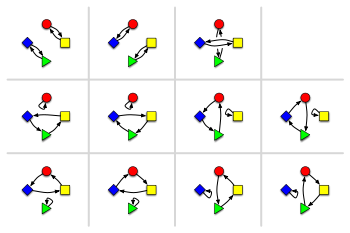
\includegraphics[scale = 0.7]{images/Stirling1.png}
        \caption{Permutations on 4 elements with 2 cycles }
        \label{Fig:StirlingI}
    \end{figure}
\subsection{Stirling numbers of the first kind (${n \brack k}$)} The number of ways of permuting $n$ elements such that the permutations have $k$ cycles is given by the Stirling number of the first kind ${n \brack k}$. Figure \ref{Fig:StirlingI} shows all possible ways of permuting 4 elements with 2 cycles (${4 \brack 2} = 11$). From the definition of ${n \brack k}$, it can clearly be seen that $$n! = \sum_{k=0}^{n} {n \brack k}$$


\Lecture{Jayalal Sarma}{Sept 29, 2020}{10}{Tutte’s Matrix Tree Theorem and counting arborescences}{Raghul}{$\alpha$}{JS}
\section{Introduction}
In this lecture, we will be looking at another application of the Principle of Inclusion-Exclusion(PIE) - Matrix Tree Theorem. We will understand the theorem and then we will cover all the bases required to prove the theorem. The proof of the theorem will be completed in the next lecture.

\section{Kirchoff’s Matrix Tree Theorem} \label{sec:kirchoff's application}
The original theorem for undirected graphs was stated by Kirchoff in the 19th century and the generalised verion for directed graphs was stated by Tutte in the 20th century. This theorem is a classical bridge between combinatorial and algebraic quantities. Let us define few important terms before we jump into the theorems and proofs.\\
\begin{definition}\textbf{Laplacian Matrix for undirected graphs:} 
For any undirected graph $G(V,E)$ with $n$ vertices, let us define a $n$x$n$ matrix $L(G)$ called the \textit{Laplacian matrix} of $G$ as follows.
\[
  L(G)_{ij} = 
  \begin{cases}
    deg(v_i) &\mbox{if }~ i = j\\
    -1 &\mbox{if }~ i \neq j ~\text{and}~(v_i,v_j)\in E\\
    0 &\mbox{otherwise}
  \end{cases}
\]
\end{definition}
\noindent
It can also be noted that for a graph $G(V,E)$ without any self edges (i.e. $\forall i, ~ (v_i,v_i) \notin E$), the Laplacian matrix can also be defined as $L(G) = D - A$ where $D$ is a diagonal matrix with $D_{ii} = ~deg(v_i)$ and $A$ is the adjacency matrix of $G$.
\begin{theorem} Matrix Tree Theorem for undirected graphs by Kirchoff:\\
For any undirected graph $G(V,E)$, the number of different spanning trees rooted at $v_i$ contained in $G$ is given by $det(L_G[i])$ where $L_G[i]$ refers to the matrix obtained by removing the $i^{\text{th}}$ row and the $i^{\text{th}}$ column from $L(G)$ (for any $i \in [n]$).
\end{theorem}
\noindent
Note that the theorem has connected a combinatorial quantity to an algebraic one. It should also be noted that $det(L_G[i])$ is the same for every value of $i$ (since the number of undirected spanning trees does not change with the root $v_i$). The usual proof of this theorem is done using induction on the number of vertices. Instead we will use PIE to prove the generalised version and this theorem will follow as a consequence. Before doing the proof, let us cover few other concepts required for the proof.
\section{Determinant of a Matrix}\label{sec:determinant of a matrix}
From high school mathematics; we all know that for a 2x2 matrix $A$ and a 3x3 matrix $B$, the determinants are given by 
\begin{align*}
  det(A) &= a_{11}a_{22}-a_{12}a_{21}\\
  det(B) &= b_{11}b_{22}b_{33}-b_{11}b_{23}b_{32}-b_{12}b_{21}b_{33}+b_{12}b_{23}b_{31}+b_{13}b_{21}b_{32}-b_{13}b_{22}b_{31}
\end{align*}
It is to be noticed that in the determinant expression of a $n$x$n$ matrix, the subscripts in each term match with one of the $n!$ possible permutations on $[n]$ and there are $n!$ terms in the expression. For example; the first term in the expression for $|A|$ represents the permutation $[1\rightarrow1; ~2\rightarrow2]$ and the other term represents $[1\rightarrow2; ~2\rightarrow1]$. Similarly, the second term in the expression for $|B|$ represents $[1\rightarrow1; ~2\rightarrow3;~3\rightarrow2]$ while the fifth term represents $[1\rightarrow3; ~2\rightarrow1;~3\rightarrow2]$.\\
Thus, each term in determinant expression of a $n$x$n$ matrix represents one of the permutations of $[n]$ and all the permutations are represented exactly once. In other words, given a permutation $\sigma$ on $[n]$, the term $\prod_{i=1}^{n} a_{i\sigma(i)}$ appears exactly once in the expression of the determinant of a $n$x$n$ matrix $A$.\\
Given any permutation $\sigma$ on $[n]$, we can represent it in the point representation as a $n$-tuple as $(\sigma(1),\sigma(2),\sigma(3)\ldots \sigma(n))$. We can define the number of inversions of $\sigma$ ($Inv(\sigma)$) as follows.
$$Inv(\sigma) = |\{(i,j)~|~i<j~\text{and}~\sigma(i)>\sigma(j)\}|$$
For example; for the permutation $\sigma_1 = (1,3,2)$, $Inv(\sigma_1) = 1$ (since (2,3) is the only such $(i,j)$ pair); for $\sigma_2 = (3,1,2)$, $Inv(\sigma_2) = 2$ (since (1,2) and (1,3) are the $(i,j)$ pairs) and for $\sigma_3 = (3,2,1)$, $Inv(\sigma_3) = 3$ (since (1,2), (2,3) and (1,3) are the $(i,j)$ pairs). \\
It can be noticed that the sign of a term representing the permutation $\sigma$ in the determinant expression is given by
$$Sign(\sigma) = (-1)^{Inv(\sigma)}$$
From the inferences done above, one can logically guess the determinant expression for a $n$x$n$ matrix $A$ in terms of
$Sign(\sigma)$ and $\prod_{i=1}^{n} a_{i\sigma(i)}$. However, until proven mathematically, this remains nothing more than a logical guess. So, let us state this as a theorem and prove it.
\begin{theorem}
For any $n \in \N$, the determinant of the $n^{\text{th}}$ order square matrix $A$ is given by
$$det(A) = \sum_{\sigma \in S_n} Sign(\sigma)  \prod_{i=1}^{n} a_{i\sigma(i)}$$
where $S_n$ is the set of all permutations on $[n]$. 
\end{theorem}
\begin{proof}
We know that the determinant of any matrix $A$ follows the following four properties.
\begin{enumerate}
    \item If all the elements in a row of $A$ are 0, then $det(A)=0$
    \item If two rows of $A$ are identical, then $det(A)=0$
    \item If a row of $A$ is a multiple of another row, then $det(A)=0$
    \item Adding the multiple of a row of $A$ to another row, does not change the value of $det(A)$
\end{enumerate}
Though not done as part of the lecture, it can be proven that there is only one expression in terms of $a_{ij}$'s that satisfies all the four properties. Therefore, it is sufficient to prove that the expression given in the theorem satisfies all the four properties stated above to prove the whole theorem. \\
Let us now prove the first property : Let all the elements in row $k$ be 0 i.e. $\forall_{j\in[n]}~ a_{kj} = 0$. It can clearly be seen that each term in the determinant expression stated in the theorem has some $a_{k\sigma(k)}$ in it. So each term will be 0 and hence $det(A)=0$. \\
Proving that the expression stated in the theorem satisfies the other three properties is left as an exercise for the students.
\end{proof}

\section{Applications of PIE} \label{sec:Applications of PIE - lec3}
\subsection{Tutte’s Matrix Tree Theorem} \label{subsec:tutte's application}
 Now, let us continue our journey towards stating and proving Tutte's Matrix Tree Theorem. Firstly, let us define Spanning Arborescences - the directed graphs equivalent for spanning trees and Laplacian matrix for directed graphs.
\begin{definition}\textbf{Spanning Arborescences:} An \textit{Arborescence} is a directed graph in which a vertex $u$ is called the root and for every other vertex $v$ in the graph, there is exactly one directed path from $u$ to $v$. In simpler terms, an arborescence is an directed tree in which all the edges are directed away from the root. A \textit{Spanning Arborescence} $S(V,E)$ of a directed graph $G(V',E')$ is an arborescence such that $V=V'$ and $E\subseteq E'$.
\end{definition}
\noindent\\
\begin{definition}\textbf{Laplacian matrix for directed graphs:} For any directed graph $G(V,E)$ with $n$ vertices, let us define a $n$x$n$ matrix $L(G)$ called the \textit{Laplacian matrix} of $G$ as follows.
\[
  L(G)_{ij} = 
  \begin{cases}
    indeg(v_i) &\mbox{if }~ i = j\\
    -1 &\mbox{if }~ i \neq j ~\text{and}~(v_i,v_j)\in E\\
    0 &\mbox{otherwise}
  \end{cases}
\]
\end{definition}
\begin{theorem} Tutte's Matrix Tree Theorem for directed graphs\\
For any directed graph $G(V,E)$, the number of different spanning arborescences rooted at $v_i$ contained in $G$ is given by $det(L_G[i])$ where $L_G[i]$ refers to the matrix obtained by removing the $i^{\text{th}}$ row and the $i^{\text{th}}$ column from $L(G)$ (for any $i \in [n]$).
\end{theorem}
\noindent
Note that since spanning arborescences are directed, the number of spanning arborecences depend on the chosen root. Hence, unlike the undirected case, $det(L_G[i])$ here depends on the value of $i$. Without loss of generality, we can choose $i = n$ for our proof. Therefore, all we should prove is the number of spanning arborescences rooted at $v_n$ for the directed graph $G$ is given by
\begin{align}
    det(L_G[n]) = \sum_{\sigma \in S_{n-1}}~
    Sign(\sigma)~\prod_{i=1}^{n-1}l_{i\sigma(i)}
    \label{eq:to_prove:Tutte}
\end{align} 
The R.H.S. of the equation is the determinant expression for the $(n-1)$x$(n-1)$ matrix $(L_G[n])$.\\Now let us define another type of directed graphs called Spregs to help with our proof process.\\
\noindent\\
\begin{definition}\textbf{Spregs:} Single prdecessor graphs or \textit{Spregs} with distinguished vertex $v$ of a directed graph $G(V,E)$ is a subgraph $T(V,E')$, $E' \subseteq E$, such that each vertex in $T$ except the vertex $v$ has exactly one predecessor and the vertex $v$ has no predecessors. In other words; in the spreg T, $indeg(v) = 0$ and for every $u \neq v$, $indeg(u)=1$.\\
\end{definition}
\begin{figure}[h]
    \centering
    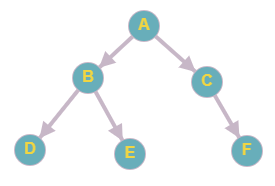
\includegraphics[scale = 0.5]{images/Spreg1.png}
    \caption{Both spreg and arborescence}
    \label{Fig:Spreg1}
\end{figure}
\begin{figure}[h]
    \centering
    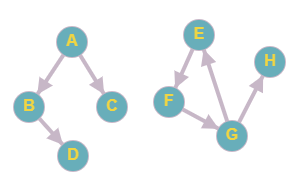
\includegraphics[scale = 0.6]{images/Spreg2.png}
    \caption{Spreg but not arborescence}
    \label{Fig:Spreg2}
\end{figure}
\noindent\\
It is important to distinguish between spregs and spanning arborescences : spregs may contain disconnected components and cycles in them. On the other hand, spanning arborescences are directed spanning trees and hence are single connected components and do not have cycles in them. The directed graph in figure \ref{Fig:Spreg1} is a spreg with distinguished vertex $A$ and an arborescence rooted at $A$. On the other hand, the graph in figure \ref{Fig:Spreg2} is a spreg with distinguished vertex $A$ but not an arborescence. Now let us consider the following lemma and prove it.
\noindent\\
\begin{lemma} If $T(V,E)$ is a spanning arborescence rooted at $v$, then $T$ is a spreg with distinguished vertex $v$.
\end{lemma}
\begin{proof}
Let $T(V,E)$ is a spanning arborescence rooted at $v$. We know from the definition that for every other vertex $u$ in $T$, there is a unique directed path from $v$ to $u$. The underlying undirected graph of $T$ is a tree and does not have any cycles and hence there should not be any cycles (directed/undirected) in $T$.\\
Let us now assume that $indeg(v) \neq 0$. This means that there exists a vertex $u$ in $T$ such that the edge $e = (u,v)\in E$. We know that there is a unique path in $T$ from $v$ to $u$ - let that path be $P$. Now the path $P+e$ is a directed cycle in $T$. A contradiction. Therefore, $indeg(v) = 0$.\\
Let us now assume that for some $u \neq v$ in $T$, $indeg(u) = 0$. This implies that T is not a spanning arborescence.  A contradiction. Therefore, $indeg(u) > 0$. \\
Let us now assume that for some $u \neq v$ in $T$, $indeg(u) \geq 2$. This implies $\exists u_1 \neq u_2$ such that $e_1 = (u_1,u) \in E$ and $e_2 = (u_2,u) \in E$. We know that there exists a unique path $P_1$ from $v$ to $u_1$ and another path $P_2$ from $v$ to $u_2$. Since $u_1 \neq u_2$, $P_1 \neq P_2$. Now, $P_1+e_1$ and $P_2+e_2$ are two distinct paths from $v$ to $u$. A contradiction. Therefore, $indeg(u) = 1$.\\
Therefore,  $indeg(v) = 0$ and for every other vertex $u$, $indeg(u) = 1$. In other words, $T$ is a spreg with distinguished vertex $v$.
\end{proof}
\noindent It is important to note that the converse of the above stated lemma is not true because spregs may contain discconnected components and cycles in them. Now, we will look at another lemma.
\noindent\\
\begin{lemma} If $T(V,E)$ is a spreg with distinguished vertex $v$, then the spreg consists of an arborescence rooted at $v$ and zero or more weakly connected components (the underlying undirected component is connected). Each of these weakly connected components have exactly one directed cycle in them.
\end{lemma}
\begin{proof}
The proof of this lemma is left as an exercise for the students to complete.
\end{proof}
\noindent Thus; (a spreg  with distinguished vertex $v$) = (an arborescence rooted at $v$) + $k$ (weakly connected components with one directed cycle each); where $k \geq 0$. \\
\noindent\\
For proving Tutte's theorem; the idea to count the number of arborescences rooted at $v_n$ is that we would count the number of spregs with distinguished vertex $v_n$ and then remove the number of spregs that are not arborescences - the terms in such a expression would exactly match with that of the R.H.S. of \ref{eq:to_prove:Tutte}.\\
\noindent\\
In the R.H.S. of \ref{eq:to_prove:Tutte}, consider the term for $\sigma =$ identity permutation i.e. $\forall i,~ \sigma(i)=i$. Clearly, $Sign(\sigma)=1$ since $Inv(\sigma)=0$. The term would be $+ \prod_{i=1}^{n-1}l_{ii}$. This is exactly equal to the total number of spregs with distinguished vertex $v_n$ - the reasoning is as follows.\\
Since $v_n$ is the distinguished vertex, ignore all the edges whose end vertex is $v_n$. For every other vertex $u$, choose exactly one of the edges whose end vertex is $u$ ($\prod_{i=1}^{n-1}indeg(v_i)$ ways). Clearly, such a subgraph is a spreg - by definition of spregs. Therefore, the number of distinct spregs is $\prod_{i=1}^{n-1}indeg(v_i) = \prod_{i=1}^{n-1}l_{ii}$ (by the definition of Laplacian matrix). \\
\noindent\\
We have counted all the spregs; now, spregs with cycles have to be removed from the count. This part of the proof involves PIE and will be done in the next lecture.

